\documentclass[tikz,border=2pt]{standalone}
\usepackage{amsmath}
\usepackage{amssymb}
\usepackage{xcolor}

\definecolor{journalink}{HTML}{1F1C18}
\definecolor{journalmuted}{HTML}{8A7F72}
\definecolor{journalaccent}{HTML}{9C2D2D}

\newcommand{\panelbox}{(-1.5,-1.5) rectangle (2.7,1.5)}
\newcommand{\circA}{(0,0) circle (1.2)}
\newcommand{\circB}{(1.2,0) circle (1.2)}

\begin{document}
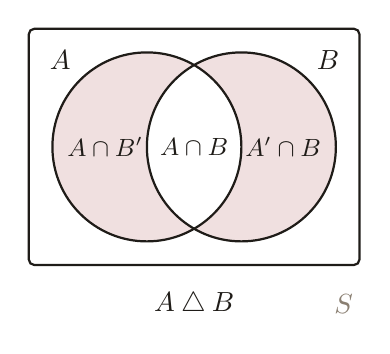
\begin{tikzpicture}[x=1cm, y=1cm, every node/.style={font=\normalsize}, accentfill/.style={fill=journalaccent, fill opacity=0.15}]

  % symmetric difference: exactly one of the two circles
  \begin{scope}[even odd rule]
    \clip \circA \circB;
    \path[accentfill] \panelbox;
  \end{scope}

  \draw[journalink, line width=0.8pt, rounded corners=2pt] \panelbox;
  \draw[journalink, line width=0.8pt] \circA;
  \draw[journalink, line width=0.8pt] \circB;
  \node[journalink, font=\small] at (-0.53,0) {$A\cap B'$};
  \node[journalink, font=\small] at (1.73,0) {$A'\cap B$};
  \node[journalink, font=\small] at (0.6,0) {$A\cap B$};
  \node[journalink] at (-1.1,1.1) {$A$};
  \node[journalink] at (2.3,1.1) {$B$};
  \node[journalink] at (0.6,-2.0) {$A\mathbin{\triangle}B$};
  \node[journalmuted] at (2.5,-2.0) {$S$};

\end{tikzpicture}
\end{document}
